%settings are located in begin_settins.tex and end_settings.tex files -> do not remove the files!
%iso-8859-2 encoding
%%% Hlavní soubor. Zde se definují základní parametry a odkazuje se na ostatní části. %%%

%% Verze pro jednostranný tisk:
% Okraje: levý 40mm, pravý 25mm, horní a dolní 25mm
% (ale pozor, LaTeX si sám přidává 1in)
\documentclass[12pt,a4paper]{report}
\setlength\textwidth{145mm}
\setlength\textheight{247mm}
\setlength\oddsidemargin{15mm}
\setlength\evensidemargin{15mm}
\setlength\topmargin{0mm}
\setlength\headsep{0mm}
\setlength\headheight{0mm}
\usepackage[utf8]{inputenc}

%% Ostatní balíčky
\usepackage{graphicx}
\usepackage{amsthm}
\usepackage{listings}

%% Balíček hyperref, kterým jdou vyrábět klikací odkazy v PDF,
%% ale hlavně ho používáme k uložení metadat do PDF (včetně obsahu).
%% POZOR, nezapomeňte vyplnit jméno práce a autora.
\usepackage[ps2pdf,unicode]{hyperref}   % Musí být za všemi ostatními balíčky
\hypersetup{pdftitle=Data Warehouse Milestone}
\hypersetup{pdfauthor=Ondrej Platek and Peteris Nikiforovs}

%%% Drobné úpravy stylu

% Tato makra přesvědčují mírně ošklivým trikem LaTeX, aby hlavičky kapitol
% sázel příčetněji a nevynechával nad nimi spoustu místa. Směle ignorujte.
\makeatletter
\def\@makechapterhead#1{
  {\parindent \z@ \raggedright \normalfont
   \Huge\bfseries \thechapter. #1
   \par\nobreak
   \vskip 20\p@
}}
\def\@makeschapterhead#1{
  {\parindent \z@ \raggedright \normalfont
   \Huge\bfseries #1
   \par\nobreak
   \vskip 20\p@
}}
\makeatother

% Toto makro definuje kapitolu, která není očíslovaná, ale je uvedena v obsahu.
\def\chapwithtoc#1{
\chapter*{#1}
\addcontentsline{toc}{chapter}{#1}
}


\def\todo#1{
\emph{\color{red} TODO: #1}
}

\def\todon#1{
  \todo{#1 \\}
}

\graphicspath{{./images/}}
\begin{document}

\pagestyle{plain}
\setcounter{page}{1}
%\tableofcontents %prida obsah





\subsection{TODO} % (fold)
\label{sub:TODO}

% subsection TODO (end)
\begin{itemize}
  \item more discuss: Discuss our strong points, our week points
  \item measures: additivity etc.
\end{itemize}

 % comment for final version
\chapwithtoc{ Data Warehousing and Data Mining}
\addtocounter{chapter}{1}
\subsection*{Task} % (fold)
\label{sub:Task}
We, Ondrej Platek and Peteris Nikiforovs, should implement and design an example data warehouse.

 % title page, content 

\chapter{Milestone - Data warehouse design} \label{cha:ml1}
    \section{Content of Milestone~\ref{cha:ml1}} 
        \label{sec:ml1_content}
    This chapter contains report from the $1^{st}$  Milestone which purpose was to design a data warehouse from chosen domain. We divided the tasks into several sections, which we now introduce.

    \section{Business Domain} \label{sec:ml1_domain}
    
The domain of this data warehouse project is a daily newspaper, modeled after The Wall Street Journal (WSJ or the Journal), which started out as a printed newspaper and later introduced an online version. It produces a daily printed edition which is delivered to subscribed customers worldwide, sold at newspaper stands. The same content is also available on the website. The online edition is available to authenticated paid subscribers only.


        \subsection{Data Warehouse Objectives} \label{sub:ml1_objectives}
         
Our company has had multiple data sources (paper receipts, paper journals, text files, proprietary binary file databases and lately SQL databases) for the print newspaper over the years which have been integrated into one relational database. 
The~online edition was designed separately and has its own databases. 

Both databases store customer data differently which makes it hard to aggregate statistics from both editions. Also, the database for the printed edition was built additively and contains data inconsistencies. The data warehouse would allow to combine personalized knowledge of the online edition readers with a lot of additional historical data from the printed edition.


WSJ is the largest newspaper in the United States by circulation and has more than 400,000 online paid subscriptions. As such, the amount of data accumulated over the years is huge and was not designed to be stored for efficient analysis. As a result, it's very inefficient to extract useful information as the business queries would take a long time when run on production databases.

The management of Journal understands, that the Web not only is a thread to printed newspaper, but also could be a huge market and source of information. As goal for new decade the Journal company is interested among others in following topics:
\begin{itemize}
    \item How to provide to advertisers guaranties and statistics that our readers will see their advertisement? (Consequently The Journal would be able to require more money from advertiser).
    \item How to arrange articles in the week in order to limit the amount of low read articles?
    \item Which articles put together in order to keep the reader reading?
    \item Find matches of convenient advertisement and articles based on pro click rate.
    \item Which advertisers we consider unimportant according our database, but have really successful campaigns and profit from our newspaper?
    \item When should we advertise the Journal to subscribers?
\end{itemize}

The WSJ decided to start building data warehouse based on the database containing new online data. Secondly, the WSJ woul like to add the~historical data to the~data warehouse. This scenario allows early result for current relevant data and it also allows incorporating historical data step by step in future.
Further on, we work only with the data collected in the online database of the WSJ.

        \subsection{Business Processes} \label{sub:ml1_processes}
        
We have identified three main business processes that such a newspaper would care about:
selling subscriptions, advertising, ensuring the quality of content.

The Journal mainly generates revenue from subscription sales. Since it is an international newspaper, It’s important to break down the sales by countries and regions. It’s also necessary for the company shareholders to visualize the growth over the years, taking into account the data from both editions.

In addition to subscriptions, the Journal places ads in the paper and generates revenue from
it. The company would like to know how much revenue it generates and compare it to the
subscription sales.

Lastly, the paper cares about the quality of its content. The Journal mainly covers economics and business topics and financial news. Since it’s possible to track all user actions on the website, the data warehouse would allow testing of introduction of new content, identifying most popular articles, determine least successful authors, etc..


        \subsection{Process Granularity} \label{sub:ml1_granularity}
        
\subsection*{Selling subscriptions} 
We break down the subscriptions by location and date in order to see how successful we are during the time on different places. It is worth to mention that subscriptions are the main source of our income. 

Highest granularity for location should be 
the~{\bf city}\footnote{In Subsection~\ref{sub:ml1_granularity} the~bold worlds  mark the finest granularity by given dimension} 
, because it is the ideal unit for describing mass behaviour.  The habits and traditions  which influences the mass behaviour are best captured on the level of cities. 

Since it's a global newspaper, countries should be grouped by regions, continents and arbitrary zones based on detail information our newspaper has about the specified region.

It's not important to know at exactly what time a subscription was purchased, but the date is relevant. 
In order to differentiate holidays, day of week we have chosen {\bf date} as our highest granularity. 

\subsection*{Advertising} 
The process of advertising is getting more important
and we want to examine advertisements according {\bf Campaigns}and date {\bf Date}.  

\subsection*{Popularity of article content} 
Since we have started with online content, we are interested which factors are crucial for popularity of our article.

We decided to measure the popularity of each article every {\bf hour}, because the reading habits of our readers probably depends on the time of a day. On the other hand, we cannot afford finer granularity because we have to store the data about all the articles.

The article popularity is probably heavily dependent on the quality and topic of the article. 
This fact we reflect by choosing the articles in finest details
according
\begin{itemize}
    \item {\bf Publication date}
    \item {\bf Subcategory of article}
    \item tags - one word description of unlimited domain (no hierarchy)
    \item {\bf Author}
\end{itemize}


 
    % section Business Domain (end)
    \clearpage

    \section{Conceptual Design of Data Warehouse}
            \label{sec:ml1_design}  
        \subsection{Facts} \label{sub:ml1_facts}
        
We present following facts according business processes from  Subsection~\ref{sub:ml1_processes}.
\begin{itemize}
    \item Advertisement - poin of view: Added at the end of a day. For each advertisement it would contain sum up information from the whole day.
    \item Subscriptions - point of view: Represent one subscription from one customer.
    \item Article popularity - point of view: Every day we store
    actual information how our articles are popular for every single article.
\end{itemize}

\begin{figure}[!hbp]
\begin{center}
  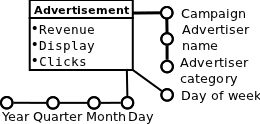
\includegraphics[scale=0.5]{fact_advertisement}
\caption{\label{pic:f_adv}  Advertisement}
\end{center}
\end{figure}

\begin{figure}[!hbp]
\begin{center}
    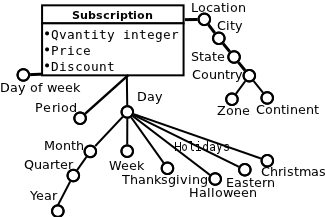
\includegraphics[scale=0.5]{fact_subscriptions}
\caption{\label{pic:f_sub}  Subscriptions}
\end{center}
\end{figure}

\begin{figure}[!hbp]
\begin{center}
  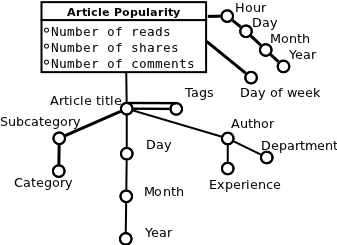
\includegraphics[scale=0.5]{fact_article}
\caption{\label{pic:f_art}  Article popularity}
\end{center}
\end{figure}


        \subsection{Fact Measures} \label{sub:ml1_measures}
        
{\bf Advertisement} fact has measures {\it Revenue},{\it Displays},{\it Clicks}. All 3 measures are additive of an integer type. All three measures could be combined to compute secondary statistic, e.g. Click rate $Clicks / Displays$. 

{\bf Subscription} is measured by {\it Price}, {\it Discount} and {\it Quantity}. The measures simply reflects the act of subscribing per one order. {\it Quantity} is number of subscriptions in one order. {\it Price} and {\it Quantity} are additive measures. {\it Discount} is proportional e.g. 0.1 meaning $10\%$ discount. It means it is not additive, however an average discount per order makes sense.

{\bf Article popularity} could be measured by {\it Number of reads}, {\it Number of shares} and {\it Number of comments}.
All three measures are additive.

All additive measures in all three facts could be sum up allong its hierachies for additional attributs. The average could be counted using {\it SUM} and {\it COUNT} on corresponding level, but realise that average of averages from disjoint subsets is not average from a the whole set.

        \subsection{Attributes and Hierarchies} \label{sub:ml1_attributes}
        

We offers different types of subscriptions based on how long the subscription last. We reflect it in attribute period.


        \subsection{Conceptual problems} \label{sub:ml1_problems}
        At first, we had difficulty identifying facts, but as we discussed business processes and made up sample business queries, we managed to identify the facts.

Secondly, we looked at facts more from a relational point of view. We did not consider evolution
of data in time, so we thought about updates in our data warehouse. Especially difficult for us was to avoid updates in facts about articles. We had originally designed the fact that had reflected only actual state. Instead of adding new information and keeping historical data, we had though about updating values in data warehouse. It was clearly wrong solution.

Finally, we managed to figure out how to designed the fact and keep the measures reads, shares and comments and also we know that the tables are sensible large.

        \clearpage
    % section Conceptual Design of Data Warehouse (end)

    \section{Logical design} 
            \label{sec:ml1_logical}
        \subsection{Star schemas} \label{sub:ml1_star}
        
\begin{figure}[!hbp]
\begin{center}
    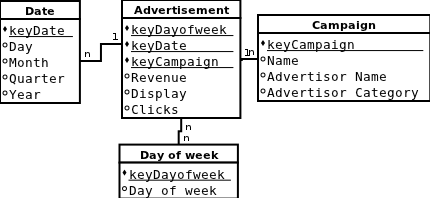
\includegraphics[scale=0.5]{schema_star_advertisement}
\caption{\label{pic:st_adv} Star schema - Advertisement}
\end{center}
\end{figure}

\begin{figure}[!hbp]
\begin{center}
    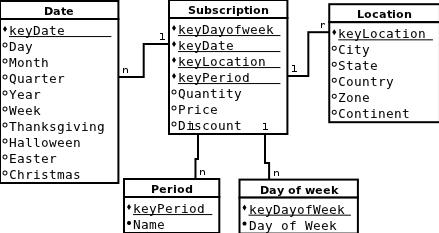
\includegraphics[scale=0.5]{schema_star_subscriptions}
\caption{\label{pic:st_sub}  Star schema - Subscriptions}
\end{center}
\end{figure}

\begin{figure}[!hbp]
\begin{center}
    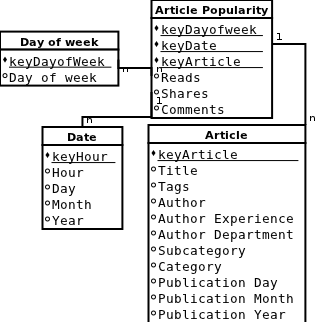
\includegraphics[scale=0.5]{schema_star_article}
\caption{\label{pic:st_art}  Star schema - Article}
\end{center}
\end{figure}


        \clearpage
        \subsection{Snowflake schemas} \label{sub:ml1_snowflake}
        
\begin{figure}[!hbp]
    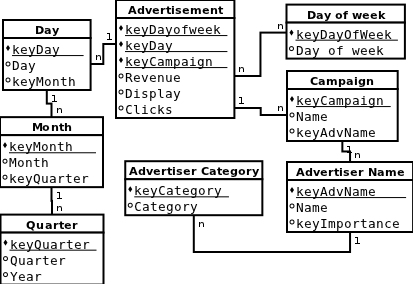
\includegraphics[scale=0.4]{schema_snowflake_advertisement}
\caption{\label{pic:sn_adv} Snowflake schema - Advertisement}
\end{figure}

\begin{figure}[!hbp]
    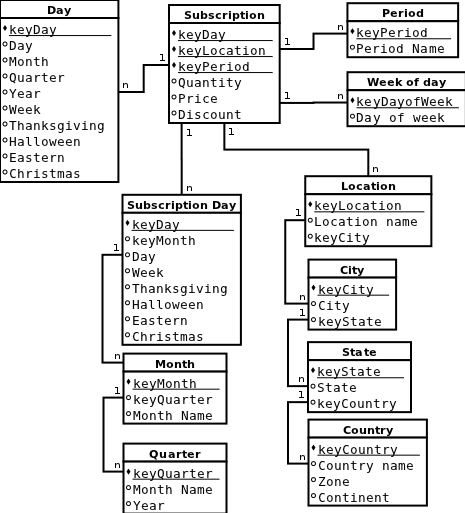
\includegraphics[scale=0.4]{schema_snowflake_subscriptions}
\caption{\label{pic:sn_sub}  Snowflake schema - Subscriptions}
\end{figure}

\begin{figure}[!hbp]
    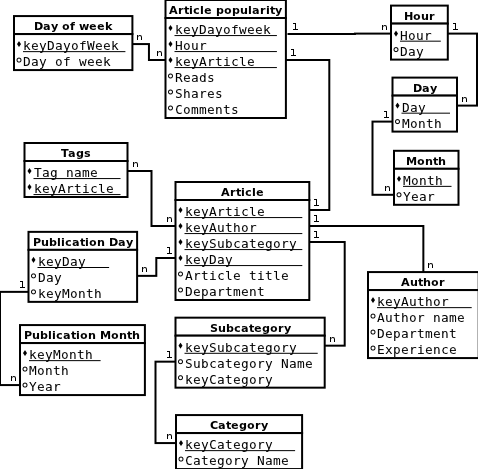
\includegraphics[scale=0.4]{schema_snowflake_article}
\caption{\label{pic:sn_art} Snowflake schema - Article}
\end{figure}

\clearpage

        \subsection{Choice between schemas} \label{sub:ml1_choice}
        
Due to the fact that our dimension tables are not so large, in sense of branching, and also they contain simple domains, the tables in star schema do not cover too much space.
 The star schema also allows better performance for data warehouse queries. In other words, the low normality of tables does not affect the space requirements too badly, because the numbers of possible values in hierarchies are relatively low.

On the other hand, the star schema allows us process aggregation function more effectively.
The aggregation functions together with joins are the key operations for data warehouse. 
The snowflake schema is in our case split in a lot of tables with relatively small number of values.
It does not save so much space compare to star schema, but only it results in sequences of joins.
To conclude, we decided to follow star schema and avoid joins in our queries as much as possible.

The only exception, which does not allow us to follow our star schema from Section~\ref{sub:ml1_star}, is the {\it Tag} attribute. 
The {\it Tag} attribute from {\it Article popularity} fact has potentially unlimited domain, because every author or editor can add arbitrary tag.  
We are using only sample data for it, but we still created a separate table for describing $n$ to $n$ relation between Tags and Articles. 
The table could be very huge and is nonsense  to make the table of {\it Article} dimension wider by another columns as it is displayed in star schema design. 

        \clearpage % for Snowflake schemas
        \subsection{Example data} \label{sub:ml1_example}
        In tables below you see sample date for a star schema introduced in~Subsection~\ref{sub:ml1_star}. As we mention in  Subsection~\ref{sub:ml1_choice} we did not used in our implementation exactly the star schema, but we separated {\it tags} attribute to another table. So notice that in our implementation we added a {\it keyTag} column in Table~\ref{t:f_artpop}, remove column {\it Tags} in  Table~\ref{t:art_dim_table} and we created {\bf separate table {\it Tags}}.
\begin{figure}[!hbp]
\caption{\label{t:f_adv}Advertisement fact table}
\begin{center}
\begin{tabular}{|c|c|c|c|c|}
\hline
keyDate & keyCampaign & Revenue & Displays & Clicks\\
\hline
\hline
874 & 32 & 20000 & 432812 & 4221\\
932 & 872 & 399 & 21322 & 213\\
\hline
\end{tabular}
\end{center}
\end{figure}

\begin{figure}[!hbp]
\caption{\label{t:adv_date}Advertisement Date dimension table}
\begin{center}
\begin{tabular}{|c|c|c|c|c|}
\hline
keyDate & Date & Month & Quarter & Year\\
\hline
\hline
874 & 23 & 1 & 1 & 2008\\
932 & 5 & 5 & 2 & 2006\\
\hline
\end{tabular}
\end{center}
\end{figure}

\begin{figure}[!hbp]
\caption{\label{t:adv_camp}Advertisement Campaign dimension table}
\begin{center}
\begin{tabular}{|c|c|c|c|}
\hline
keyCampaign & Name & Advertiser Name & Advertiser Category\\
\hline
\hline
32 & 2012 Volkswagen CC Ad & Volkswagen & Big Fish\\
872 & Free Lunch at Mensa & Bolzano University & Small Fish\\
\hline
\end{tabular}
\end{center}
\end{figure}

\begin{figure}[!hbp]
\caption{\label{t:f_sub}Subscription fact table}
\begin{center}
\begin{tabular}{|c|c|c|c|c|c|}
\hline
keyDate & keyLocation & keyPeriod & Quantity & Price & Discount\\
\hline
\hline
423 & 2311 & 1223 & 2 & 100.58 & 0.1\\
43 & 88 & 8898 & 10 & 920.3 & 0.1\\
\hline
\end{tabular}
\end{center}
\end{figure}

\begin{figure}[!hbp]
\caption{\label{t:sub_date}Subscription date dimension table}
\begin{center}
\begin{tabular}{|c|c|c|c|c|c|p{1.3cm}|p{1.2cm}|p{1.3cm}|p{1cm}|}
\hline 
keyDate &Date&Month&Quarter& Year & Week & Thanks- giving & Eastern & Christ- mas & Hallo- ween\\
\hline
\hline
423 & 31 & 10 & 4 & 2011 & 1 & 0 & 0 & 0 & 1\\
43 & 24 & 12 & 4 & 2005 & 6 & 0 & 0 & 1 & 0\\
\hline
\end{tabular}
\end{center}
\end{figure}


\begin{figure}[!hbp]
\caption{\label{t:sub_loc|}Subscription location dimension table}
\begin{center}
\begin{tabular}{|c|c|c|c|c|c|}
\hline
keyLocation & City & State & Country & Zone & Continent\\
\hline
\hline
2311 & New York & New York & United States & US and Canada & North America\\
88 & Bolzano & South Tyrol & Italy & Southern Europe & Europe\\
\hline
\end{tabular}
\end{center}
\end{figure}

\begin{figure}[!hbp]
\caption{\label{t:sub_per}Subscription period dimension table}
\begin{center}
\begin{tabular}{|c|c|c|}
\hline
keyPeriod & Name & Order\\
\hline
\hline
1223 & Month& 3\\
8898 & Annual& 5\\
\hline
\end{tabular}
\end{center}
\end{figure}

\begin{figure}[!hbp]
\caption{\label{t:f_artpop}Article Popularity fact table}
\begin{center}
\begin{tabular}{|c|c|c|c|c|}
\hline
keyDate & keyArticle & Reads & Shares & Comments\\
\hline
\hline
2011020117 & 1000 & 212 & 20 & 5\\
2011020118 & 1000 & 53 & 2 & 4\\
\hline
\end{tabular}
\end{center}
\end{figure}

\begin{figure}[!hbp]
\caption{\label{t:art_date}Article Popularity Date dimension table}
\begin{center}
\begin{tabular}{|c|c|c|c|c|}
\hline
keyDate  & Hour & Date & Month & Year\\
\hline
\hline
2011020117 & 17 & 02 & 11 & 2011\\
\hline
2011020118 & 18 & 02 & 11 & 2011\\
\hline
\end{tabular}
\end{center}
\end{figure}


\begin{figure}[!hbp]
\caption{\label{t:art_dim_table}Article Popularity dimension table }
\begin{center}
\begin{tabular}{|p{1cm}|p{1cm}|p{1cm}|p{1.25cm}|p{1.25cm}|p{1.25cm}|p{1.35cm}|p{1.3cm}|p{0.7cm}|p{1.05cm}|p{0.9cm}|}
\hline
key Article & Title & Tags & Author & Author Exp. & Author Dept. & Sub category & Cate- gory & Pub. Day & Pub. Month & Pub. Year\\
\hline
\hline
1000 & Article  & rude funny & John Smith & Junior Reporter & Enter- tainment & Fashion & Life and Style & 02 & 11 & 2011\\
\hline
9999 & Wake the economy & serious actual&Jane Doe & Senior Reporter & Finance & Earnings & Business & 03 & 11 & 2011\\
\hline
\end{tabular}
\end{center}
\end{figure}

        \clearpage
%force to print all figures
    % section Logical design (end)

    \section{SQL Implementation} % (fold)
    \label{sec:implementation}
    
Our data was generated partially randomly and partially randomly chosen from public databases.
Firstly, we created the populating scripts for PostgresSQL 9.1. Lately, we decided to migrate
our database to Oracle 10.2.0.3.0, because Postgres does not support data mining extensions.
We had to modify the populating scripts to fit Oracle syntax and also subdivide them,
because Oracle does not support some commands with our permissions, e.g. "CREATE SCHEMA" command.

We divided generated data into several SQL scripts which creates tables, populates tables, and delete tables.
We provide init.sh file. It allows to populate database, see Figure~\ref{l:ml1_init}, and also deleting the tables, see Figure~\ref{l:ml1_drop}.
\begin{figure}[!hbp]
\begin{lstlisting}[language=bash]
$ cd init
# comment: init connects to database granted to us from school
# comment: for more information check the script itself
$ ./init.sh init login password
# it will take quite about 4 hours to populate the data
\end{lstlisting}
\caption{Populating data warehouse using  init.sh script} \label{l:ml1_init}
\end{figure}

\begin{figure}[!hbp]
\begin{lstlisting}[language=bash]
$ cd init
# comment: droping the table/ removing the data warehouse 
# comment: still from init directory
$ ./init.sh drop login password
\end{lstlisting}
\caption{Removing data warehouse using  init.sh script} \label{l:ml1_drop}
\end{figure}

For more details about SQL scripts, the init.sh script or the script for generating data view the source code of the scripts, it should be self explenatory. In enclosed README.txt we list all containing scripts and the usage again.

\subsection*{Data}
To generate the SQL scripts for populating the database we used PHP scripts enclosed.

We created some data artificially, for some we used real world data.
It is worth to note that we used real address data from Canada and also we filled the tags with a few samples from real tags from real Wall Street Journal.

% subsection Data (end)


% chapter Milestone 1 (end)

\chapter{Milestone - Data warehouse querying} \label{cha:ml2}
    \section{Content of Milestone~\ref{cha:ml2}} 
        \label{sec:ml2_content}
    
\subsection*{Task} % (fold)
\label{sub:name}
For the designed data warehouse write 20 aggregation queries in both natural language and SQL. Include the results (if the resulting data amount is big, include a sample).
% subsection Task (end)


    \section{Business queries} \label{sec:ml2_queries}
    \section{Business queries} % (fold)
\label{sub:Business queries}

\subsection*{Task} % (fold)
\label{sub:name}
For the designed data warehouse write 20 aggregation queries in both natural language and SQL. Include the results (if the resulting data amount is big, include a sample).
% subsection Task (end)

\subsection*{Subscription queries} % (fold)
\label{sub:Subscription business queries}
\begin{enumerate}
  \item Revenue from subscriptions by year.
\begin{lstlisting}[language=sql]
select sum(price * (1-discount) * quantity) revenue, d.year 
from sub_subscription s 
join sub_date d on s.keydate = d.keydate 
group by d.year 
order by year desc
\end{lstlisting}
  \item Which were the most popular subscription periods each year?
\begin{lstlisting}[language=sql]
select year, p.name as period, sum(quantity) subscriptions
from oplatek.sub_subscription s 
join oplatek.sub_date d on s.keydate = d.keydate
join oplatek.sub_period p on s.keyperiod = p.keyperiod 
group by d.year, p.name
order by year desc, subscriptions desc
\end{lstlisting}
  \item Revenue from subscriptions and subscription count by country in 2010.
\begin{lstlisting}[language=sql]
select l.country, sum(price * (1-discount) * quantity) revenue, 
  sum(quantity) subscriptions 
from oplatek.sub_subscription s 
join oplatek.sub_location l on s.keylocation = l.keylocation 
join oplatek.sub_date d on s.keydate = d.keydate and d.year = 2010
group by l.country 
order by revenue desc
\end{lstlisting}
  \item Top 10 cities from each country with the highest revenue from subscriptions in 2010.
\begin{lstlisting}[language=sql]  
select * from (select country, city, 
  sum(price * (1-discount) * quantity) revenue, 
  rank() over(partition by country 
    order by sum(price * (1-discount) * quantity) desc) rank 
from oplatek.sub_subscription s 
join oplatek.sub_date d 
  on s.keydate = d.keydate and d.year = 2010
join oplatek.sub_location l 
  on s.keylocation = l.keylocation
group by l.country, l.city
order by revenue desc)
where rank <= 10
\end{lstlisting}
  \item How much would we earn without applying discounts on subscriptions, by period type and by year?
\begin{lstlisting}[language=sql] 
select year, period, revenue, revenue_no_discounts, 
  (revenue_no_discounts - revenue) difference from 
    (select d.year, p.name as period, 
      sum(price * (1-discount) * quantity) revenue, 
      sum(price * quantity) revenue_no_discounts
     from oplatek.sub_subscription s 
     join oplatek.sub_date d on s.keydate = d.keydate
     join oplatek.sub_period p on s.keyperiod = p.keyperiod
     group by d.year, p.name)
order by year desc, period asc
\end{lstlisting}
  \item Number of sales on different holidays by period in Canada in 2010.
\begin{lstlisting}[language=sql] 
TODO
select country, year, period, total_sales, 
(select sum(quantity) from 
    oplatek.sub_subscription ss, oplatek.sub_date dd 
 where ss.keydate = dd.keydate and dd.christmas = 'Y' 
  and ss.keyperiod = p.keyperiod 
  and ss.keylocation = l.keylocation) as christmas,
 from (select l.country, d.year, p.name period, sum(quantity) total_sales
 from oplatek.sub_subscription s 
 join oplatek.sub_date d on s.keydate = d.keydate and d.year = 2010
 join oplatek.sub_location l on s.keylocation = l.keylocation and l.country = 'Canada'
 join oplatek.sub_period p on s.keyperiod = p.keyperiod 
 group by l.country, d.year, p.name)
order by d.year, period
\end{lstlisting}
  \item Revenue by month and by state in Canada in 2010 together with average revenue by states in Canada in the same month.
\begin{lstlisting}[language=sql] 
select l.state, d.month, 
  sum(price * (1-discount) * quantity) revenue,
  /* avg_revenue_in_this_month_across_all_states */
  avg(sum(price * (1-discount) * quantity)) 
    over (partition by month) avg_rev 
from oplatek.sub_subscription s 
join oplatek.sub_location l 
    on s.keylocation = l.keylocation and l.country = 'Canada' 
join oplatek.sub_date d 
    on s.keydate = d.keydate and d.year = 2010
where length(l.state) = 2
group by l.state, d.month
order by state asc, month asc
\end{lstlisting}
\end{enumerate}
% subsection Subscription queries (end)

\subsection*{Article queries} % (fold)
\label{sub:Article  queries}
\begin{enumerate}
\item    Top 10 read articles and their authors for every month in year 2011.
\begin{lstlisting}[language=sql] 
select * from (
 select d.month, a.keyarticle as id, 
  a.title, a.author, sum(reads) reads, 
  rank() over (partition by month order by sum(reads) desc) rank 
 from oplatek.artpop_articlepopularity f
 join oplatek.artpop_article a on f.keyarticle = a.keyarticle
 join oplatek.artpop_date d on f.keydate = d.keydate 
     and d.year = 2010
 group by d.month, a.keyarticle, a.title, a.author
 order by month asc, reads desc
) where rank <= 10
\end{lstlisting}
\item    Hours of the day when most articles are read grouped by category in year 2010 together with the average number of articles read during this hour in the same year.
\begin{lstlisting}[language=sql] 
select a.category, d.hour, sum(reads) reads, 
    avg(sum(reads)) over (partition by hour) avg_reads 
from oplatek.artpop_articlepopularity f
join oplatek.artpop_article a on f.keyarticle = a.keyarticle
join oplatek.artpop_date d on f.keydate = d.keydate 
    and d.year = 2010
group by a.category, d.hour
order by a.category asc, d.hour asc
\end{lstlisting}
\item    Number of articles published in each subcategory in year 2010 together with the % of total articles in the category.
\begin{lstlisting}[language=sql] 
select category, subcategory, articles/sum(articles) over (partition by category) perct, articles, sum(articles) over (partition by category) as articles_in_category from (
select a.category, a.subcategory, count(a.keyarticle) articles
from oplatek.artpop_articlepopularity f
join oplatek.artpop_article a on f.keyarticle = a.keyarticle and a.publicationyear = 2011
group by a.category, a.subcategory
order by category, subcategory
)
\end{lstlisting}
\item    Top 5 authors in every category by comments on their articles.
\begin{lstlisting}[language=sql] 
select * from (
select a.category, a.author, sum(comments) comments, 
  rank() over (partition by a.category 
    order by sum(comments) desc) rank 
from oplatek.artpop_articlepopularity f
join oplatek.artpop_article a on f.keyarticle = a.keyarticle
group by a.category, a.author
order by a.category asc, comments desc
) where rank <= 5
\end{lstlisting}
\item    Each author's 5 most read articles with the number of total article reads together with the average number of article reads for this author's department and each author must have at least 20 articles published, all these articles must have been published before 2011 and total reads for each article must be above the average article read count for the author's department.
\begin{lstlisting}[language=sql] 
select *
from (select a.author, 
  rank() 
    over (partition by a.author order by sum(reads) desc) rank,
  a.keyarticle id, a.title,
  sum(reads) reads, 
  a.authordepartment department,
  avg(sum(reads)) 
    over (partition by a.authordepartment) deparment_reads,
  count(a.keyarticle) 
    over (partition by a.author) total_articles
from oplatek.artpop_articlepopularity f
join oplatek.artpop_article a on f.keyarticle = a.keyarticle
where a.publicationyear < 2011
group by a.author, a.authordepartment, a.keyarticle, a.title
order by a.author, rank asc)
where rank <= 5 and reads > deparment_reads 
and total_articles >= 20
\end{lstlisting}
\item    Top 20 articles published in October, 2011 with the \#comments/\#reads higher than the average \#comments/\#reads having at least 20000 \#reads.
\begin{lstlisting}[language=sql] 
select * from (
select a.keyarticle id, a.title,
   sum(reads)/sum(comments) comm_by_reads,
   avg(sum(reads)/sum(comments)) over () avg_comm_by_reads,
   sum(reads) reads
from oplatek.artpop_articlepopularity f
join oplatek.artpop_article a on f.keyarticle = a.keyarticle
where a.publicationyear = 2011 
and a.publicationmonth = 10
group by a.keyarticle, a.title
order by comm_by_reads - avg_comm_by_reads desc
) where comm_by_reads > avg_comm_by_reads 
and reads >= 20000 and rownum <= 20
\end{lstlisting}
\item    Compare the number of reads/shares/comments of articles tagged with positive and negative tags for each year.
\begin{lstlisting}[language=sql] 
select year, tag, 
reads, sum(reads) over (partition by year) reads_total, reads/sum(reads) over (partition by year) reads_perc,
reads, sum(shares) over (partition by year) shares_total, shares/sum(shares) over (partition by year) shares_perc,
reads, sum(comments) over (partition by year) comments_total, comments/sum(comments) over (partition by year) comments_perc
from (
select a.publicationyear year, t.tag, sum(reads) reads, sum(comments) comments, sum(shares) shares
from oplatek.artpop_articlepopularity f
join oplatek.artpop_article a on f.keyarticle = a.keyarticle
join oplatek.artpop_tag t on t.tag in ('positive', 'negative')
join oplatek.artpop_articletags artt on a.keyarticle = artt.keyarticle and artt.keytag = t.keytag 
group by a.publicationyear, t.tag
order by year desc, tag
)
\end{lstlisting}
\item   Top 100 tags by article count in Business category in 2011.
\begin{lstlisting}[language=sql] 
select rank() over (order by count(a.keyarticle) desc) rank, t.tag, count(a.keyarticle) articles
from oplatek.artpop_articlepopularity f
join oplatek.artpop_article a on f.keyarticle = a.keyarticle and a.category = 'Business' and a.publicationyear = 2011
join oplatek.artpop_tag t on 1=1
join oplatek.artpop_articletags artt on a.keyarticle = artt.keyarticle and artt.keytag = t.keytag
group by t.tag
order by rank, tag asc
\end{lstlisting}
\end{enumerate}
% subsection Article  queries (end)

\subsection*{Advertisement  queries} % (fold)
\label{sub:Advertisement queries}

\begin{enumerate}
\item    Revenue by year together with average revenue in all years together with revenue in this year and together with next year
\begin{lstlisting}[language=sql] 
select ad.Year, sum(aa.revenue), 
  avg(sum(aa.revenue)) over () as total_avg,
  sum(sum(aa.revenue)) over 
    (order by ad.year rows 1 preceding) as sum_last_2_years
from   
advert_advertisement aa
join advert_date ad on aa.keydate = ad.keydate
group by ad.YEAR;
  \end{lstlisting}
\item    CPM(Clicks divided by displays) for top 10 advertisers by revenue together with avg CPM for advertisers category having the advertiser at least 15 campaigns
  \begin{lstlisting}[language=sql] 
select *
from 
(    select
        rank() over (order by sum (aa.revenue) desc) as top,
        sum(aa.clicks)/sum(aa.displays),ac.advertiserName,
        ac.advertiserCategory as cat, 
        avg(sum(aa.clicks)/sum(aa.displays)) 
            over (partition by ac.advertiserCategory)
    from advert_advertisement aa
    join advert_campaign ac on aa.keycampaign = ac.keycampaign
    join
      ( select distinct in_aa.advertiserName 
        from advert_campaign in_aa
        group by in_aa.advertiserName
        having COUNT(in_aa.name) >= 15
      )
    camp on ac.advertiserName = camp.advertiserName
    group by rollup (ac.advertiserName,ac.advertiserCategory) 
    having grouping_id(ac.advertiserName,ac.advertiserCategory)=0
    )
where 
top < 10;
\end{lstlisting}
\item Revenue by advertiser from "Small Fish" category who has greater revenue than average of the "Middle Fish"*bias=0.5 together with average of "Middle Fish" advertisers  
  \begin{lstlisting}[language=sql] 
select ac.advertiserName, ac.advertiserCategory, sum(aa.revenue), 
 avg(sum(aa.revenue)) over (partition by ac.advertiserCategory) 
 as small_fish_avg,
 ( 
  select distinct
   AVG(sum(aaa.revenue)) over 
    (partition by aac.advertiserCategory) as middle_fish_avg
    from advert_advertisement aaa 
    join advert_campaign aac on aaa.keycampaign = aac.keycampaign
    where aac.advertiserCategory = 'Medium Fish'   
    group by aac.advertiserName,aac.advertiserCategory
  ) as middle_fish_avg
from advert_advertisement aa
join advert_campaign ac on aa.keycampaign = ac.keycampaign
where ac.advertiserCategory = 'Small Fish'
group by ac.advertiserName,ac.advertiserCategory
having sum(aa.revenue) > 0.5* (
  -- having is stupid, I have to repeat query:)
  select distinct
    AVG(sum(aaa.revenue)) over (partition by aac.advertiserCategory) 
    as middle_fish_avg
  from advert_advertisement aaa 
  join advert_campaign aac on aaa.keycampaign = aac.keycampaign
  where aac.advertiserCategory = 'Medium Fish'   
  group by aac.advertiserName,aac.advertiserCategory);
  \end{lstlisting}
\item    The Campaigns which touched more than 5 month with maximum revenue in one month bigger than 140 all in year 2011 
  \begin{lstlisting}[language=sql] 
select * from (
  select ac.name, max(sum(aa.revenue)) 
    over (partition by ac.name) as max_revenue_over_month
  from advert_advertisement aa
  join advert_date ad on ad.keyDate = aa.keyDate
  join advert_campaign ac on ac.keyCampaign = aa.keyCampaign
  where ad.year=2011
  group by ac.name, ad.month
  having ( max(ad.month) - min(ad.month)) >= 0 
    or ( (max(ad.month) - min(ad.month)) = 5 
    and (max(ad.day) - min(ad.day)) >=0 )
) where max_revenue_over_month > 140;
  \end{lstlisting}
\item Most popular campaigns by year together with their popularity(clicks+displays) and  avg CPM per month
  \begin{lstlisting}[language=sql] 
select y, c, n, popularity, cpm_per_month
from (
  select ad.year y, ac.name n,  ad.month, ac.advertisercategory c
  , sum(aa.clicks+aa.displays) popularity
  ,(avg(sum(aa.clicks)/sum(aa.displays)) 
    over (partition by ad.month)) cpm_per_month 
  from advert_advertisement aa
  join advert_date ad on ad.keyDate = aa.keyDate
  join advert_campaign ac on ac.keyCampaign = aa.keyCampaign
  group by ad.month,ad.year, ac.name,ac.advertisercategory
  )
order by y desc, c, popularity desc, n;

  \end{lstlisting}
\end{enumerate}
% section Business queries (end)

% section Advertisement business queries (end)

    \subsubsection{Ranking queries} % (fold)
\label{ssub:Ranking queries}
We have enclosed our ranking queries in list of business queries at Subsection~\ref{sec:ml2_queries}.
See queries Subscription query number $4$, from Article queries numbers $2$, $4$, $5$
and query $2$ from Advertisement section
% subsubsection Ranking queries (end)

\subsection{Windowin queries} % (fold)
\label{sub:Windowin queries}
Number of windowing queries (queries using windowing functions with the"{\it OVER}" statement)
could be found also Subsection~\ref{sec:ml2_queries}.
Let us name queries $2$ and $5$ from Article section or queries $1$, $2$, $3$, $4$ from Advertisement part.
% subsection Windowin queries (end)

\subsection{Period-to-Period queries} % (fold)
\label{sub:Period-to-Period queries}
%    \begin{itemize}
%        \item Difference between number of reads of article on the publication date and the date in one week and the date in 2 weeks
%        \item Total revenue from subscriptions in last 3 years
%    \end{itemize}
\begin{itemize}
    \item Revenue from subscriptions by year and week compared to the revenue on the same week in the previous year.
\begin{lstlisting}[language=sql] 
select year, week, revenue, 
 sum(revenue) over (partition by week order by year 
  RANGE BETWEEN 1 PRECEDING AND 1 PRECEDING) 
  revenue_last_year_this_week        
from (
 select 
  year, week, sum(price * (1-discount) * quantity) revenue 
 from oplatek.sub_subscription s 
 join oplatek.sub_date d on s.keydate = d.keydate 
 group by d.year, d.week)
order by year desc, week asc;
\end{lstlisting}

\item Revenue from subscriptions by year and week compared to the average revenue on the same week in the 3 previous years.
\begin{lstlisting}[language=sql] 
select year, week, revenue, avg(revenue) 
 over (partition by week order by year 
       RANGE BETWEEN 3 PRECEDING AND 1 PRECEDING) 
       avg_revenue_prev_3_years        
from (
select year, week, 
 sum(price * (1-discount) * quantity) revenue 
from oplatek.sub_subscription s 
join oplatek.sub_date d on s.keydate = d.keydate
group by d.year, d.week)
order by year desc, week asc;
\end{lstlisting}

\end{itemize}
% subsection Period-to-Period queries (end)

\subsection{Dense reports} % (fold)
\label{sub:Dense reports}
\begin{itemize}
\item Revenue from subscriptions by year.
\begin{lstlisting}[language=sql] 
select b.year, NVL(revenue, 0)  dense_revenue from (
select year, sum(price * (1-discount) * quantity) revenue 
from oplatek.sub_subscription s 
join oplatek.sub_date d on s.keydate = d.keydate 
group by d.year 
order by year desc
) a
right outer join (
  select distinct dd.year
  from oplatek.sub_date dd
) b on (a.year = b.year)
order by b.year desc;
\end{lstlisting}

\item Number of articles published in 1999 in each category.
\begin{lstlisting}[language=sql] 
select b.category, b.subcategory, NVL(articles,0) dense_articles 
from (
 select a.category, a.subcategory, count(a.keyarticle) articles
 from oplatek.artpop_articlepopularity f
 join oplatek.artpop_article a 
  on f.keyarticle = a.keyarticle and a.publicationyear = 1999
 group by a.category, a.subcategory
 order by category
) a
right outer join (
  select distinct aa.category, aa.subcategory
  from oplatek.artpop_article aa
) b 
on (a.category = b.category and a.subcategory = b.subcategory)
order by category, subcategory;
\end{lstlisting}
\end{itemize}

% subsection Dense reports (end)

    \section{Execution plan} % (fold)
    \label{sec:exec_plan}
    
We have chosen fact Subscription for implementing materialized views and indexes.
We will implement materialised views for queries number $3$ $4$ and $7$ from Subscription part of Section~\ref{sec:ml2_queries}.

The three above mentioned queries are good candidates for materialized view because they aggregate heavily and gives relative small results based on lot of data.
   
Also for indexes is this fact interesting because the queries $3$ and $4$ use "where" clause on columns with no indexes so implementing indexes will result in better performance.
 
Last but definitely not least, we suppose that Subscription fact would be the most queried fact from our data warehouse.

It is worth to mention that we decided to choose third query for impementing indexes for fact article popularity to see the difference. The main reason is the fact has $1 672 252$ rows, so should be able to see the performance improvement easily.

    \subsection{Materialized views} \label{sub:ml2_views}
    
In our queries we do not use dimensions {\it Period Name} and {\it Day of week}, but 
we use {\it Date} hierarchy and {\it Location} hierarchy. 
In order to discuss, which materialised views should we implement we will use Lattice framework to describe dependencies. We will denote the size of views directly in the lattice diagram for relevant views.

 The "{\it group by}" sets needed to answer all 3 queries are represented by all nodes except the node representing the finest granularity. So the candidate views cover the whole lattice except the top most node on Figure~\ref{fig:lattice}. 

%All of 3 queries use aggregation function below over groups specified in Table~\ref{t:groupby}.
%\begin{lstlisting}[language=sql] 
%sum( price * (1-discount ) * quantity )
%\end{lstlisting}

\begin{figure}[!hbp]
\caption{\label{t:groupby}Attributes in group by statement from our 3 queries}
\begin{center}
\begin{tabular}{|p{3cm}|p{3cm}|p{5cm}|}
\hline
Query 3 & Query 4 & Query  7\\
\hline
\hline
Country & City, State  & State, Month\\
\hline
\end{tabular}
\end{center}
\end{figure}

 All views which has at least the same level of aggregation as our chosen 3 queries in one attribute are relevant candidates for materialised views. Unfortunately, aggregation of our 3 queries (See Figure~\ref{t:groupby}) covers almost whole 
 lattice.\footnote{The lattice represents the level of aggregation}. So we have to decide among large number of candidates.

We have created 3 materialised views~\ref{s:view_co},~\ref{s:view_ci} and~\ref{s:view_m_s}.
The views are denoted in Figure~\ref{fig:lattice}.
See the lattice legend to find out that ${Co}$ means that
the view is grouped by a country.
Queries in Figures~\ref{s:requery_3},~\ref{s:requery_4} and~\ref{s:requery_7} use the views and correspond to queries $3$, $4$ and $7$.

\begin{figure}[!hbp]
\begin{lstlisting}[language=sql] 
create materialized view view_co 
build immediate  as
select l.country, 
  sum( s.price * (1-s.discount)  * s.quantity ) s_revenue,
  sum(quantity) s_subscriptions
from sub_subscription s
join sub_date d on s.keyDate = d.keyDate
join sub_location l 
  on s.keyLocation = l.keyLocation and d.year=2010
group by l.country; 
\end{lstlisting}
\caption{\label{s:view_co} Materialized view $\{Co\}$ grouped by $country$}
\end{figure}
(
We have decided to store in our views all ready precomputed aggregation values, because the computed 
measure $revenue$ is additive. It arise a possibility to use a View from Figure~\ref{s:view_ci} in rewritten queries~\ref{s:requery_3} and~\ref{s:requery_4}, because we aggregate along location hierarchy.
The table below describes performance improvements for separate views. 

\begin{tabular}{|l|c|c|c|c|c|}
\hline
View & Rows in View & Size$[MB]$ & Query 3$[s]$ & Query 4$[s]$ & Query 7$[s]$\\
\hline
\hline
No view & 0 & - & 0.018 & 0.031 & 0.109 \\
$\{S,M\}$ & $|Month|*|State|$ & 0.0625 & - & - & 0.056\\
$\{Ci\}$ & $|City|$ & 0.0625 & !0.9!- & 0.18 & -\\
$\{Co\}$ & $|Country|$ &0.0625 & 0.01 & - & -\\
\hline
\end{tabular}

The value for view $\{Ci\}$ and query $4$ is marked with exclamation marks, 
because it does not return complete results. We included it to explore how the performance change 
using different level of aggregation in views. In the summary at the end of this subsection we stress,
that we can afford not to reuse the vies, because there are ridiculously small.

During writing the queries using views, we realised that star schema does not allow easily combine "grouped-by" tables from different dimensions easily. In fact, to use two separate views with aggregated values by $month$ and in second view aggregated values by $state$, we would be forced to join the dimension tables of $location$ and $date$ containing the whole hierarchies.

Such table is bigger than join of the $fact table$ with the $date$ and $location$ dimension, so it is nonsense to use it.
If we had implemented snowflake schema, the we can join more tables along hierarchies but only with the key values,
so it would make sense to measure the performance in that case.


\begin{figure}[!htp]
\begin{lstlisting}[language=sql] 
----- rewriten for view_co ->0.02s
select s_revenue, s_subscriptions from view_co 
order by s_revenue desc;
----- rewritten for  view_ci 
-- BAD RESULTS ->PERFORMANCE TEST ONLY
select l.country, sum(ci_revenue) revenue from
view_ci
join sub_location l on l.city = view_ci.city
group by country
order by revenue;
\end{lstlisting}
\caption{\label{s:requery_3} Rewritten queries for $3$. query}
\end{figure}

\begin{figure}[!hbp]
\begin{lstlisting}[language=sql] 
create materialized view view_ci 
build immediate as
select l.city, sum( s.price * (1-s.discount)  * s.quantity ) ci_revenue  
from sub_subscription s
join sub_date d on s.keyDate = d.keyDate
join sub_location l on s.keyLocation = l.keyLocation and d.year=2010
group by l.city;
\end{lstlisting}
\caption{\label{s:view_ci} Materialized view $\{Ci\}$ grouped by $city$}
\end{figure}

\begin{figure}[!hbp]
\begin{lstlisting}[language=sql] 
-- rewritten for view_ci --0.018
select * from (
 select l.country, l.city, max(ci_revenue),  
  rank() over(partition by country 
    order by sum(ci_revenue) desc) rank1 
 from view_ci 
 join sub_location l on view_ci.city = l.city
 group by l.country, l.city
 order by max(ci_revenue) desc)
where rank1 <=10;
\end{lstlisting}
\caption{\label{s:requery_4} Rewritten query for $4$. query}
\end{figure}

\begin{figure}[!hbp]
\begin{lstlisting}[language=sql] 
create materialized view view_m_s 
build immediate  as
select l.state, d.month, 
  sum( s.price * (1-s.discount)  * s.quantity ) m_s_revenue,
  avg(sum(price * (1-discount) * quantity)) 
    over (partition by month) m_s_avg_rev
  from sub_subscription s
join sub_date d on s.keyDate = d.keyDate
join sub_location l on s.keyLocation = l.keyLocation
where d.year=2010
group by l.state, d.month; 
\end{lstlisting}
\caption{\label{s:view_m_s} Materialized view $\{M_S\}$ grouped by $month$ and $state$}
\end{figure}

\begin{figure}[!hbp]
\begin{lstlisting}[language=sql] 
select * from view_m_s
order by state asc, month asc;
\end{lstlisting}
\caption{\label{s:requery_7} Rewritten query for $7$. query}
\end{figure}



%Let us firstly present some numbers.
%\begin{itemize}
%    \item Subscription fact table has 44632 rows
%    \item Join of fact table and {\it location} dimension has 4463200 rows (all queries)
%    \item Join of fact table and {\it date} dimension 163085328          (query 7)
%\end{itemize}
%Size of one rows on disc space is:
%http://www.datadisk.co.uk/html_docs/oracle/views.htm
%\begin{itemize}
%    \item 
%\end{itemize} %We have decided to use materialised

\begin{figure}[!htp]
\begin{center}
  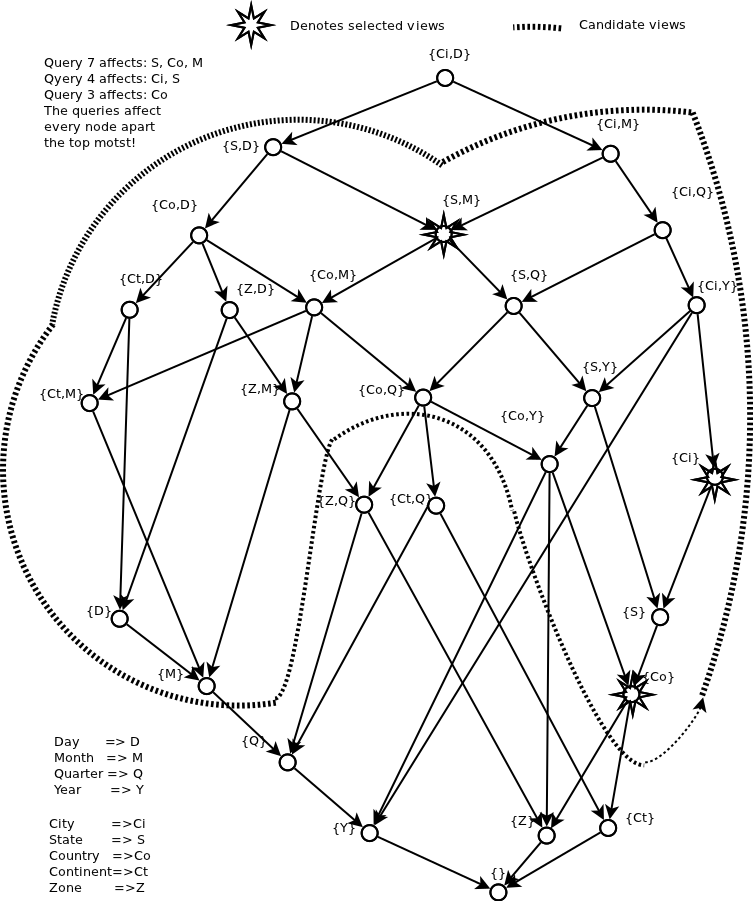
\includegraphics[scale=0.45]{lattice}
\caption{\label{fig:lattice}  Lattice}
\end{center}
\end{figure}

\subsection*{Summary} 
To conclude, this section about choosing and implementing materialised views we would like to stress some observation
which we have learned from our data.
\begin{itemize}
    \item For queries which {\bf aggregates heavily} and which has results a few rows, it {\bf always} pays of to use materialised views. In our example it is views $\{S,M\}$ and $\{Co\}$ see table above.
    \item All our Views including does not exceeds the smallest default block allocated by Oracle 
        \footnote{We used table $user\_extents$ to determine size of tables. See section $1)$ in Figure~\ref{s:details}.}
    \item Views speed up queries a lot, but if you do reuse the views in different queries,
    caching is probably easier alternative and works really well.
    \item Due to caching we have to "rename" our queries, 
    because we did not have sufficient privileges to turn caching off\footnote{
        See commands in section $2)$ in Figure~\ref{s:details}.}
    \item During design phase possibility of integrating views in star or snowflake schema should play role
    in deciding between snowflake and star schema.
    \item Oracle is capable of finding out itself that we used materialized views. 
    (We have to specify\footnote{See section $3)$ in Figure~\ref{s:details}.} it during creation.)
    On the other hand, it is not working very well, so basically you have to rewrite your queries.
\end{itemize}

\begin{figure}[!hbp]
\begin{center}
\begin{lstlisting}[language=sql] 
-- 1) determinig size of view or table
select segment_name table, sum(bytes)/(1024*1024) size_MB
from user_extents where segment_type='TABLE'
and segment_name = '&name' group by segment_name;

-- 2) disabling caching 1. method
ALTER SYSTEM FLUSH BUFFER_CACHE;
-- 2) disabling caching 2. method
ALTER TABLESPACE oplatek OFFLINE;

-- 3) enables rewriting the queries by using this views
create materialized view view_co 
    build immediate   --not relevant here
    enable query rewrite --this is important
    ...
\end{lstlisting}
\caption{\label{s:details}Technical details}
\end{center}
\end{figure}

    \clearpage
    \subsection{Indexes} \label{sub:ml2_indexes}
    \subsection*{Task} 
Check what types of indexes does Your DBMS support. Name and describe those of them which are especially useful for speeding up Your
queries.

Oracle 10g provides several indexing schemes
\footnote{\url{http://docs.oracle.com/cd/B19306_01/server.102/b14231/indexes.htm}}
that provide complementary performance functionality. These are:
\begin{itemize}
\item B-tree indexes: the default and the most common
\item B-tree cluster indexes: defined specifically for cluster
\item Hash cluster indexes: defined specifically for a hash cluster
\item Global and local indexes: relate to partitioned tables and indexes
\item Reverse key indexes: most useful for Oracle Real Application Clusters applications
\item Bitmap indexes: compact; work best for columns with a small set of values
\item Function-based indexes: contain the precomputed value of a function/expression
\item Domain indexes: specific to an application or cartridge.
\end{itemize}

A B-tree is a tree data structure that keeps data sorted and allows searches, sequential access, insertions, and deletions in logarithmic time. It is designed to allow quickly finding those tuples that have a specific key value. For this reason, they are suitable for speeding up selection operations. 

We will use B-trees to index primary keys and other columns which are used to filter data.

Bitmap indexes are also designed for finding tuples by a specific key but are very structurally different from B-tree indexes. A bitmap index is like two-dimensional boolean arrays of the same size as the number of rows for every value where each element contains a binary value indicating whether the row contains this value. In this structure, the binary value takes up only 1 bit and for each possible value the number of rows bits are used. It is much more space efficient than B-trees if the number of possible values is very low. Another feature of bitmap indexes is the ability to quickly do index intersections.

In our data warehouse we have several columns which contain only a small set of possible values. By using bitmap indexes for these columns, it is possible to reduce the storage space taken up by the indexes. When a query filters data with several of these columns at the same time, the database system will combine these indexes to return data very quickly.


\subsection*{Task} 
For the chosen queries and their versions which use the materialized views,
implement indexes to improve their performance (You can try to evaluate
several strategies and choose the best one, e.g. best speed/size ratio).
Argue Your choice. Describe the overhead (index size, computation time,
index update costs, etc.) of implementing the chosen indexes

The following formulas to calculate the size of indexes are used: 
\begin{itemize}
    \item B-Tree index: $(NK*len(k)+NR*len(r))/(D*u)$ \footnote{
Shortcuts used: $NK$ = number of distinct key values, NR = 1000000 number of relations, len(k) = key length in kilobytes, len(r) = RID (disk page and location) length in kilobytes, D = 4096 disk page size in kilobytes, u = 1 fill factor for leaves}
    \item Bitmap index: $(NR/D*8)*NK$
\end{itemize}

\begin{lstlisting}[language=sql]
select l.country, sum(price * (1-discount) * quantity) revenue, 
  sum(quantity) subscriptions 
from oplatek.sub_subscription s 
join oplatek.sub_location l on s.keylocation = l.keylocation 
join oplatek.sub_date d on s.keydate=d.keydate and d.year=2010
group by l.country 
order by revenue desc
\end{lstlisting}

There should be B-tree indexes on $sub_subscription$. $ keyLocation$ and $sub_location.keyLocation$. Bitmap indexes are not suitable for this because there are many possible values and such a bitmap index would take up much more space.
\begin{itemize}
\item Index size: $(1000000*8+1000000*8)/(4096*1) = 21.48 MB$ (30.52 GB for bitmap indexes)
\item Computation time: $O(log n)$
\item Update cost:$O(log n)$
\end{itemize}

There should be an index of $(keyDate, year)$ on $sub_date$. Assuming 365 days per year and 100 years $\rightarrow$ 36500 tuples. 36 thousands values is not considered a small set which would be suitable for bitmap. 

    
    % section execution plan (end)

% chapter Milestone 2 (end)

%\chapter{Milestone 3} \label{cha:ml3}
% todo include it

% chapter Milestone 3 (end)

%do not remove!
\end{document}

